% !TEX TS-program = xelatex
% !TEX encoding = UTF-8 Unicode
% !Mode:: "TeX:UTF-8"

\documentclass{resume}
\usepackage{array}
\usepackage{graphicx}
\usepackage{setspace} % provides onehalfspacing environment
\usepackage{cite}

\begin{document}
\pagenumbering{gobble} % suppress displaying page number

\name{Resume}

\basicInfo{
  \email{zhoulukai329@gmail.com} \textperiodcentered\
  \phone{(+86) 189-3991-4215} \textperiodcentered\
  \github{https://github.com/zhoulukai329-spec}
}

\section{\texorpdfstring{{\normalfont\faInfo}\ }{}Personal Profile}

\noindent
\begin{minipage}[t]{0.80\textwidth}
\vspace{0pt}
\small
\begin{spacing}{1.04}
\addfontfeatures{LetterSpace=0.8}
\setlength{\tabcolsep}{0pt}
\renewcommand{\arraystretch}{1.05}
\begin{tabular}{@{}>{\raggedright\arraybackslash}p{0.19\linewidth}@{\hspace{0.7em}}>{\raggedright\arraybackslash}p{0.77\linewidth}@{}}
Name: & Zhou Lukai \\
Gender: & Male \\
Date of Birth: & March 29, 2006 \\
Education: & Undergraduate (Class of 2028) \\
Major: & Cyberspace Security \\
Phone/WeChat: & +86 18939914215 (WeChat ID: zlk94hhz) \\
AI Experience: & Long-term follower and user of mainstream large language models such as ChatGPT, Claude, and Gemini; familiar with their differences in information retrieval, reasoning and analysis, content generation, and code assistance;\\
&Long-term follower and user of specialized models such as YOLO and Sora, with an understanding of their use cases;\\
&Experienced in LLM API integration, open-source model deployment, and Agent workflow development; regularly uses AI coding tools such as Codex and Trae to assist with development, debugging, and demo validation;\\
&Experienced in Prompt Engineering, capable of designing role settings, output constraints, and iterative optimization based on task objectives, and organizing experimental processes into structured solution documentation.\\

\end{tabular}
\end{spacing}
\end{minipage}\hfill
\begin{minipage}[t]{0.16\textwidth}
\vspace{0pt}
\raggedleft
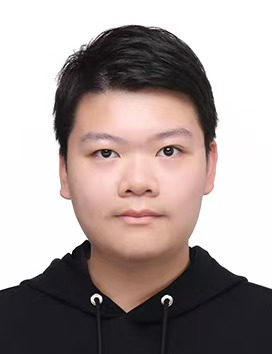
\includegraphics[width=\linewidth,height=0.18\textheight,keepaspectratio]{photo.jpg}
\end{minipage}


\section{\texorpdfstring{{\normalfont\faGraduationCap}\ }{}Education}
\datedsubsection{\textbf{Xiamen University}}{Sep. 2024 -- Present}
\textit{Bachelor's Degree}\ in Cyberspace Security, expected graduation June 2028\\
Relevant Coursework and Performance: Principles of Artificial Intelligence, Computer Networks, Principles of Operating Systems, C Programming (A), Algorithm Design and Analysis (A), Probability and Statistics (A), Principles of Database Systems (B+), Elective: AI Agents and Workflow Automation (B+)

\section{\texorpdfstring{{\normalfont\faUsers}\ }{}Project Experience}
\datedsubsection{\textbf{AI Agent-based Database Deduplication Project Using LangChain}}{Mar. 2026 -- May 2026}
\role{Python, LangChain}{Team Project (Collaboration with BlackBerry)}
Designed an AI Agent-assisted deduplication solution to address database redundancy caused by duplicate user registrations, and completed the Agent workflow design and evaluation validation\\
\begin{onehalfspacing}
https://github.com/Fovir-GitHub/ccoe\\
Key Contributions:
\begin{projectitems}
  \item Designed and implemented an AI Agent-based database deduplication and evaluation pipeline starting from real-world deduplication scenarios, establishing the main workflow of ``data preprocessing - feature generation - similarity judgment - result evaluation''
  \item Implemented the AI Agent reasoning process using the LangChain architecture, encapsulating steps such as embedding generation and data standardization as Tools to support autonomous invocation by the Agent based on task needs
  \item Performed data preprocessing and standardization in Python, generating vector representations via API calls or locally deployed models through Ollama, and validated the deduplication pipeline
  \item Built a standardized fingerprint generation logic based on fields such as name, email, company, and course, comparing the original dataset with the deduplicated result set to establish a four-category offline evaluation system (TP, FP, TN, FN)
  \item Conducted threshold sensitivity experiments in the range of 0.85--0.95 focusing on false deletions and missed detections, identifying the optimal threshold range as [0.88, 0.92]; achieved a Precision of approximately 0.83 and Recall of approximately 0.92 at a threshold of 0.90
\end{projectitems}
\end{onehalfspacing}
\projectdivider

\datedsubsection{\textbf{AI Agent and Reinforcement Learning System for Complex Rule-based Tasks}}{Jun. 2026 -- Present}
\role{PyTorch, Reinforcement Learning, CNN, ReAct}{Collaborative Project}
Designed and implemented an AI Agent system with a closed loop of perception, decision-making, and execution for various mini-games with complex and unknown rules, aiming to improve the model's autonomous reasoning capability in unknown tasks\\
https://github.com/zhoulukai329-spec/arc-intelligence-agent.git (This project is not yet open-sourced due to an ongoing related competition; it will be open-sourced once the competition concludes)\\
Key Contributions:
\begin{onehalfspacing}
\begin{projectitems}
  \item Designed and implemented the main reinforcement learning pipeline of ``feature extraction + trial-and-error policy learning + training and evaluation'', completing a closed-loop model from state to action decision
  \item Constructed general state features based on signals such as color distribution, centroid position, action masks, progress ratio, and inter-frame changes from the game UI, supporting shared policy learning across tasks
  \item Implemented a lightweight Policy Gradient-style training framework, including training/validation splitting, epsilon-greedy exploration, discounted return updates, and advantage optimization
  \item Designed a layered ``eyes-brain-hands'' collaborative architecture, decoupling perception encoding, rule reasoning, action planning, execution verification, and memory modules to improve system maintainability
  \item Built a reward mechanism and offline evaluation pipeline with continuous parameter tuning, optimizing agent behavior quality and generalization ability through step penalties, progress rewards, repeated-state penalties, and terminal rewards
\end{projectitems}
\end{onehalfspacing}
\projectdivider

\datedsubsection{\textbf{Gomoku Battle Game Based on Neural Networks, Reinforcement Learning, and PPO Optimization}}{May 2026 -- Jun. 2026}
\role{Python, PyTorch, RL, CNN, PPO}{Individual Project}
\begin{onehalfspacing}
An intelligent Gomoku battle game
\\https://github.com/zhoulukai329-spec/Gomoku\_Master\_for\_SOF106
\begin{projectitems}
  \item Implemented a PPO Actor-Critic agent for Gomoku using PyTorch, adopting 3-channel board encoding, residual CNN feature extraction, and a dual-headed Policy/Value network, supporting 15x15 board state modeling and move decision-making
  \item Designed a self-play training pipeline incorporating legal move masking, temperature control, reward shaping, gradient clipping, and checkpoint-based match evaluation to improve training stability
  \item Replaced the traditional Policy Gradient method with PPO policy optimization to improve the efficiency and stability of policy updates
  \item Added a bootstrap monitoring mechanism to prevent users from directly using an untrained model, which could otherwise lead to abnormal model behavior
\end{projectitems}
\end{onehalfspacing}


% Reference Test
%\datedsubsection{\textbf{Paper Title\cite{zaharia2012resilient}}}{May. 2015}
%An xxx optimized for xxx\cite{verma2015large}
%\begin{itemize}
%  \item main contribution
%\end{itemize}

\section{\texorpdfstring{{\normalfont\faCogs}\ }{}Technical Skills}
% increase linespacing [parsep=0.5ex]
\begin{itemize}[parsep=0.5ex]
  \item Programming Languages: Python, C/C++, Golang, MySQL, Java
  \item Operating Systems: Windows, Linux
  \item AI / Frameworks: PyTorch, LangChain, Ollama, Huggingface model deployment and API integration
  \item AI Tools: ChatGPT, Claude, Gemini, Codex, Trae
  \item Version Control: Git, GitHub
  \item Containerization: Docker
  \item Product Skills: Requirements breakdown, PRD writing
\end{itemize}

\section{\texorpdfstring{{\normalfont\faHeartO}\ }{}Awards}
\datedline{Mathematical Contest in Modeling (MCM/ICM), \textit{Finalist Nomination}}{Feb. 2026}

\section{\texorpdfstring{{\normalfont\faInfo}\ }{}Additional Information}
% increase linespacing [parsep=0.5ex]
\begin{itemize}[parsep=0.5ex]
  \item GitHub: https://github.com/zhoulukai329-spec
  \item Languages: English - Proficient (studied abroad during undergraduate studies; able to read AI product/technical documentation in English)
\end{itemize}

%% Reference
%\newpage
%\bibliographystyle{IEEETran}
%\bibliography{mycite}
\end{document}